\documentclass[11pt]{article}
\usepackage[textwidth=18.0cm, textheight=23.0cm, top=2.0cm]{geometry}
\usepackage{pst-all}
\usepackage{amssymb}
\usepackage{tikz}
\usepackage{underscore}\begin{document}
\pagestyle{empty}


ClassName: \underline{\textbf{Class_10.2bp-21}}
\par
BinSize: \underline{\textbf{100 × 100}}
\par
ReduceSize: \underline{\textbf{100 × 100}}
\par
TypeNum: \underline{\textbf{59}}
\par
Num: \underline{\textbf{60}}
\par
OutS: \underline{\textbf{120000}}
\par
InS: \underline{\textbf{108960}}
\par
Rate: \underline{\textbf{0.908}}
\par
UB: \underline{\textbf{12}}
\par
LB0: \underline{\textbf{12}}
\par
LB: \underline{\textbf{12}}
\par
LBWithCut: \underline{\textbf{12}}
\par
NodeCut: \underline{\textbf{0}}
\par
ExtendedNodeCnt: \underline{\textbf{1}}
\par
GenNodeCnt: \underline{\textbf{1}}
\par
PrimalNode: \underline{\textbf{0}}
\par
ColumnCount: \underline{\textbf{12}}
\par
TotalCutCount: \underline{\textbf{0}}
\par
RootCutCount: \underline{\textbf{0}}
\par
LPSolverCnt: \underline{\textbf{1}}
\par
PricingSolverCnt: \underline{\textbf{0}}
\par
BranchAndBoundNum: \underline{\textbf{1}}
\par
isOpt: \underline{\textbf{true}}
\par
TimeOnPrimal: \underline{\textbf{0.000 s}}
\par
TimeOnPricing: \underline{\textbf{0.000 s}}
\par
TimeOnRmp: \underline{\textbf{0.063 s}}
\par
TotalTime: \underline{\textbf{0.125 s}}
\par
\newpage


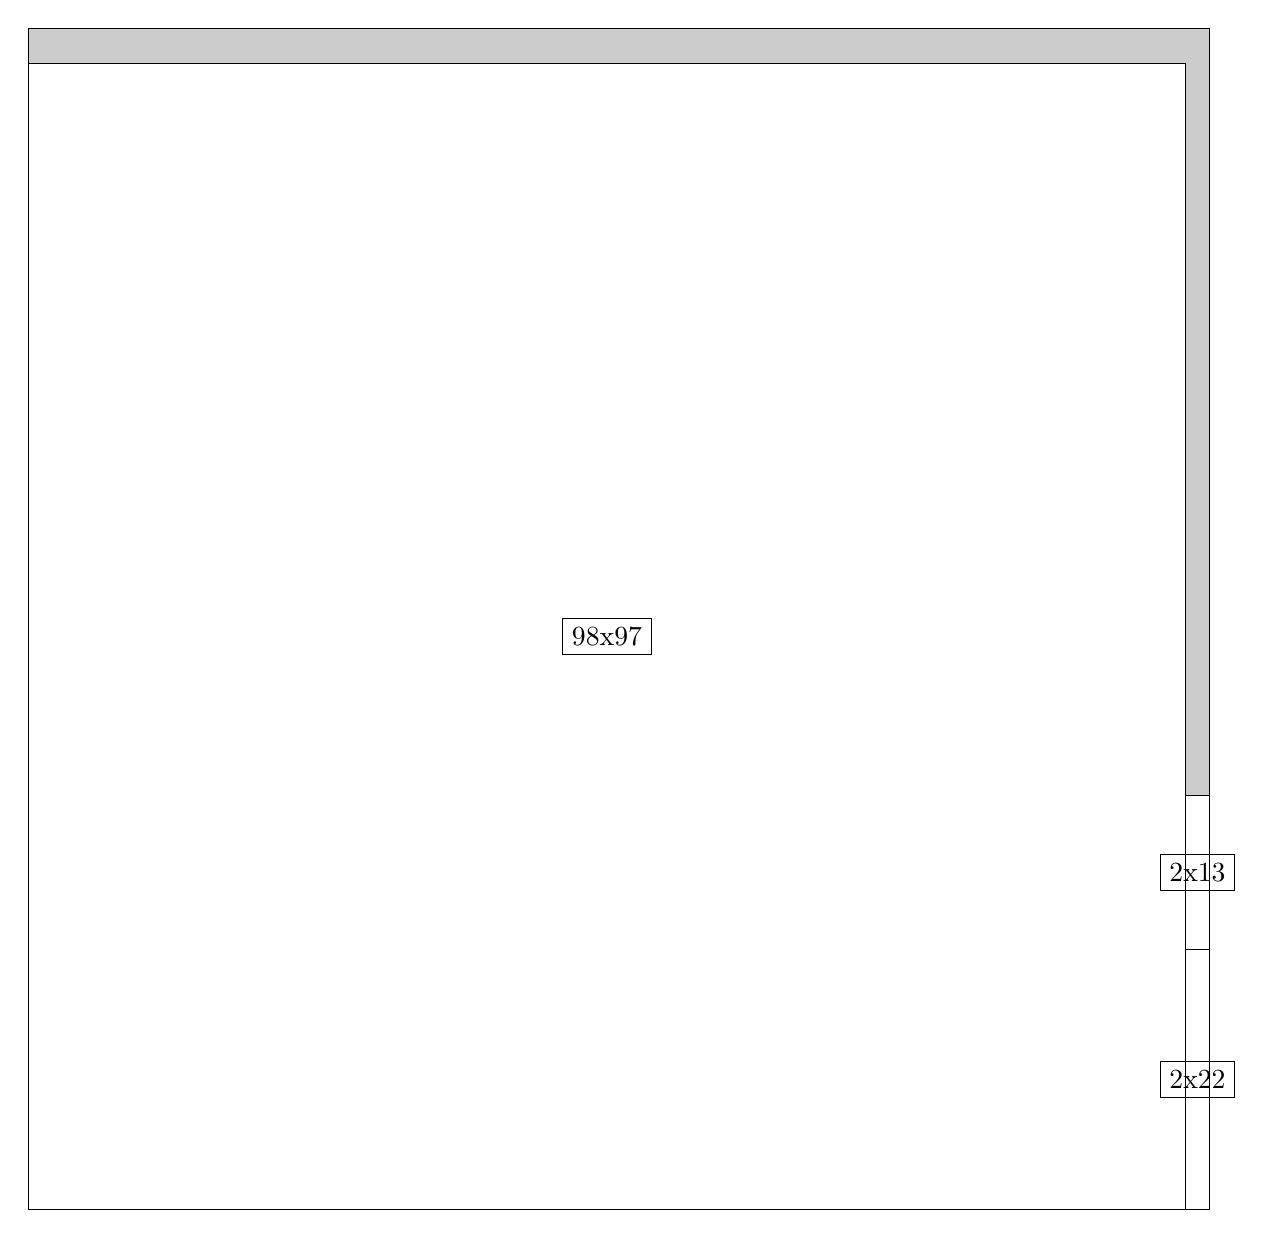
\begin{tikzpicture}[shorten >=1pt,scale=1.0,every node/.style={scale=1.0},->]
\tikzstyle{vertex}=[circle,fill=black!25,minimum size=14pt,inner sep=0pt]
\filldraw[fill=gray!40!white, draw=black] (0,0) rectangle (15.0,15.0);
\foreach \name/\x/\y/\w/\h in {98x97/0.0/0.0/14.7/14.549999999999999,2x22/14.7/0.0/0.3/3.3,2x13/14.7/3.3/0.3/1.95}
\filldraw[fill=white!40!white, draw=black] (\x,\y) rectangle node[draw] (\name) {\name} ++(\w,\h);
\end{tikzpicture}


w =98 , h =97 , x =0 , y =0 , v =9506
\par
w =2 , h =22 , x =98 , y =0 , v =44
\par
w =2 , h =13 , x =98 , y =22 , v =26
\par
\newpage


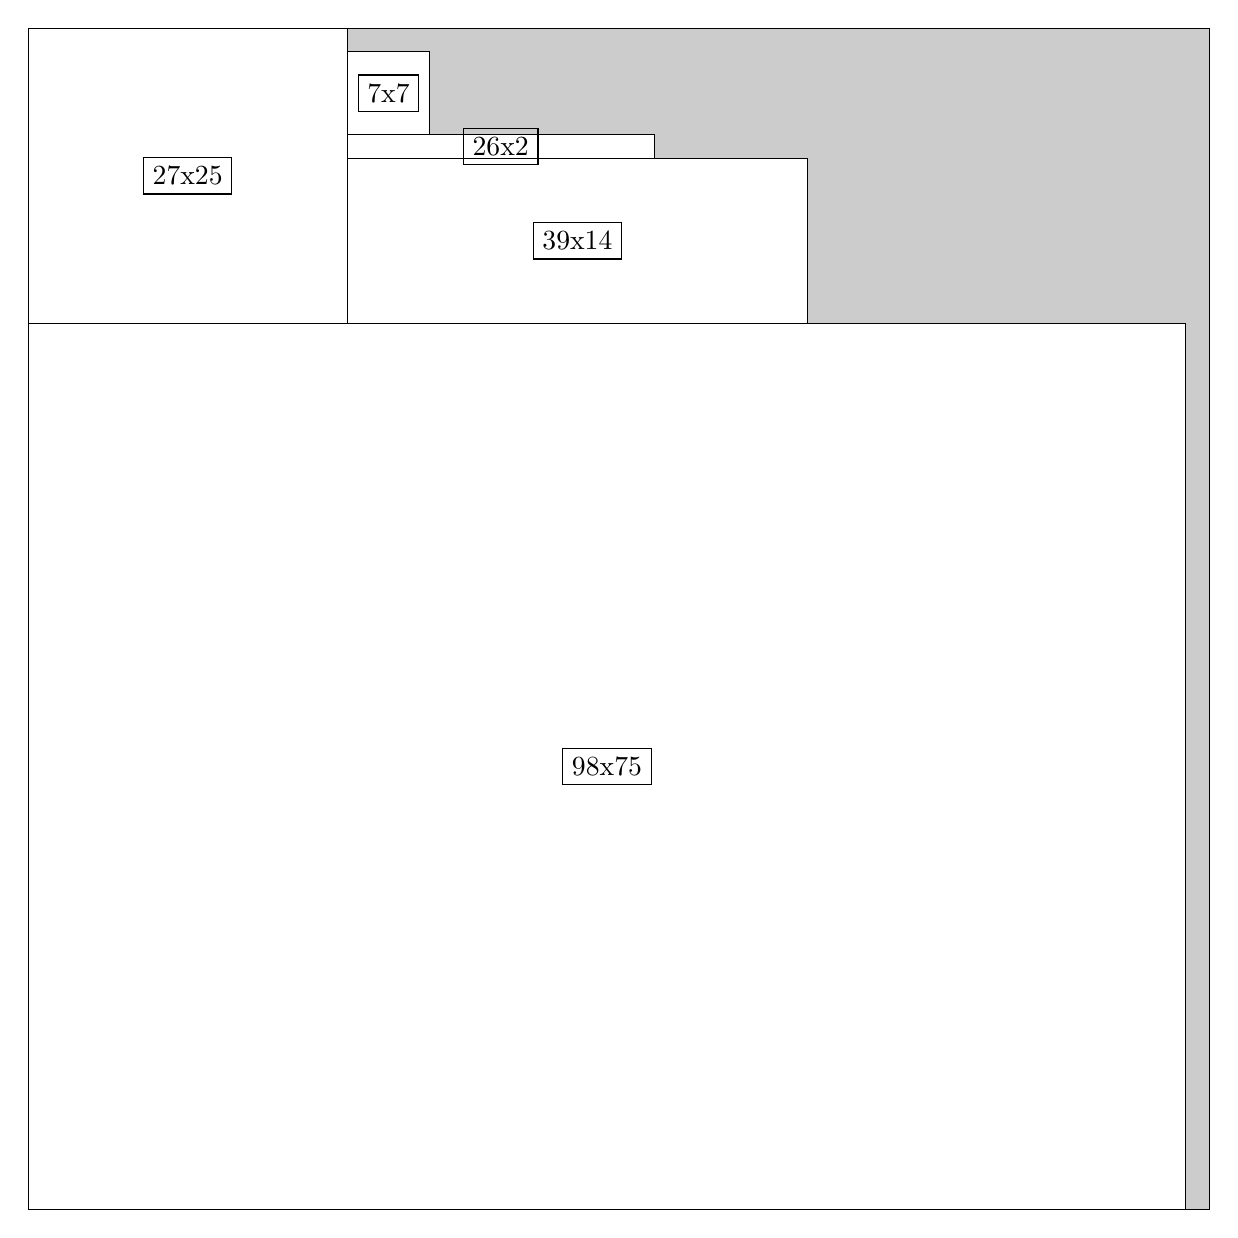
\begin{tikzpicture}[shorten >=1pt,scale=1.0,every node/.style={scale=1.0},->]
\tikzstyle{vertex}=[circle,fill=black!25,minimum size=14pt,inner sep=0pt]
\filldraw[fill=gray!40!white, draw=black] (0,0) rectangle (15.0,15.0);
\foreach \name/\x/\y/\w/\h in {98x75/0.0/0.0/14.7/11.25,27x25/0.0/11.25/4.05/3.75,39x14/4.05/11.25/5.85/2.1,26x2/4.05/13.35/3.9/0.3,7x7/4.05/13.65/1.05/1.05}
\filldraw[fill=white!40!white, draw=black] (\x,\y) rectangle node[draw] (\name) {\name} ++(\w,\h);
\end{tikzpicture}


w =98 , h =75 , x =0 , y =0 , v =7350
\par
w =27 , h =25 , x =0 , y =75 , v =675
\par
w =39 , h =14 , x =27 , y =75 , v =546
\par
w =26 , h =2 , x =27 , y =89 , v =52
\par
w =7 , h =7 , x =27 , y =91 , v =49
\par
\newpage


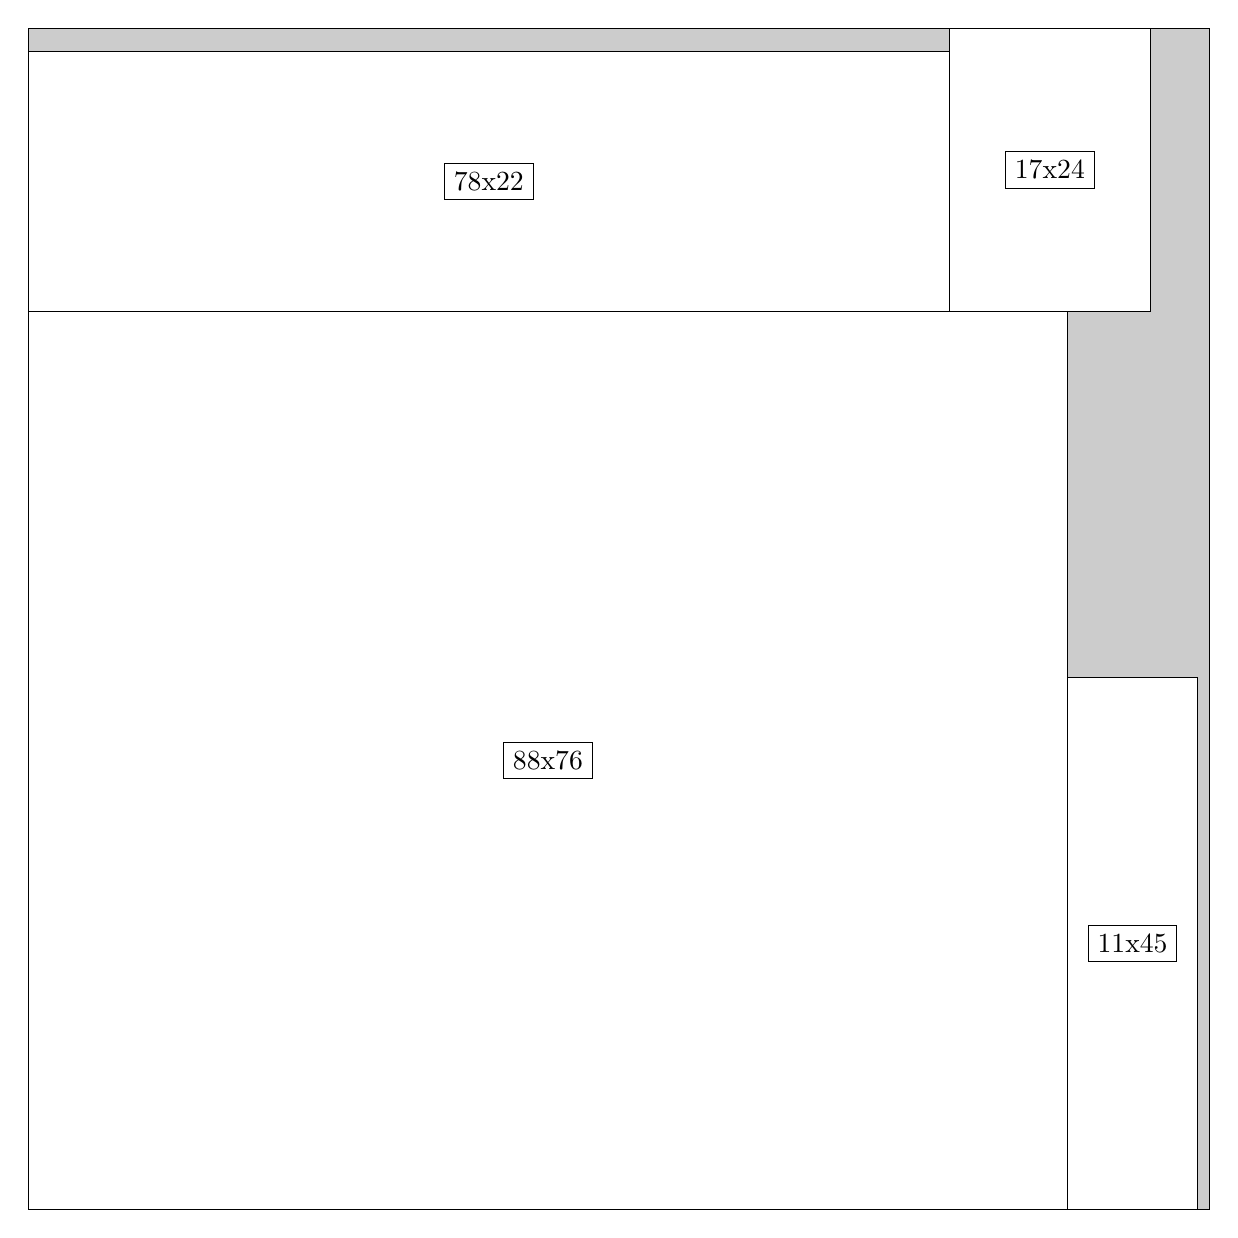
\begin{tikzpicture}[shorten >=1pt,scale=1.0,every node/.style={scale=1.0},->]
\tikzstyle{vertex}=[circle,fill=black!25,minimum size=14pt,inner sep=0pt]
\filldraw[fill=gray!40!white, draw=black] (0,0) rectangle (15.0,15.0);
\foreach \name/\x/\y/\w/\h in {88x76/0.0/0.0/13.2/11.4,78x22/0.0/11.4/11.7/3.3,11x45/13.2/0.0/1.65/6.75,17x24/11.7/11.4/2.55/3.5999999999999996}
\filldraw[fill=white!40!white, draw=black] (\x,\y) rectangle node[draw] (\name) {\name} ++(\w,\h);
\end{tikzpicture}


w =88 , h =76 , x =0 , y =0 , v =6688
\par
w =78 , h =22 , x =0 , y =76 , v =1716
\par
w =11 , h =45 , x =88 , y =0 , v =495
\par
w =17 , h =24 , x =78 , y =76 , v =408
\par
\newpage


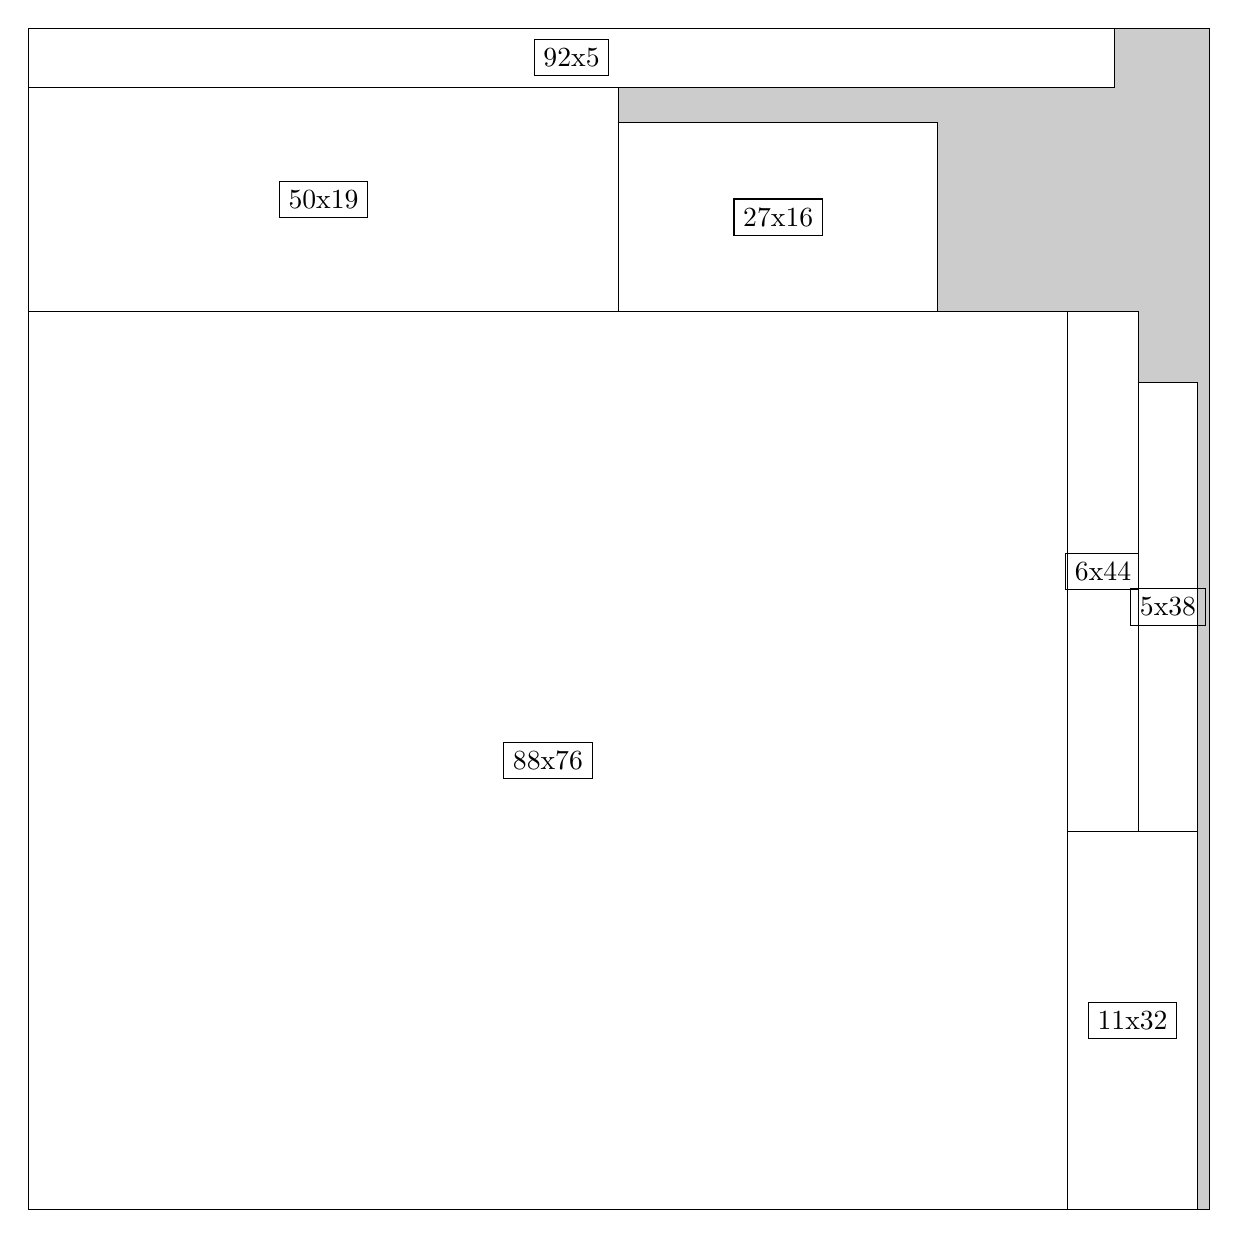
\begin{tikzpicture}[shorten >=1pt,scale=1.0,every node/.style={scale=1.0},->]
\tikzstyle{vertex}=[circle,fill=black!25,minimum size=14pt,inner sep=0pt]
\filldraw[fill=gray!40!white, draw=black] (0,0) rectangle (15.0,15.0);
\foreach \name/\x/\y/\w/\h in {88x76/0.0/0.0/13.2/11.4,50x19/0.0/11.4/7.5/2.85,92x5/0.0/14.25/13.799999999999999/0.75,27x16/7.5/11.4/4.05/2.4,11x32/13.2/0.0/1.65/4.8,6x44/13.2/4.8/0.8999999999999999/6.6,5x38/14.1/4.8/0.75/5.7}
\filldraw[fill=white!40!white, draw=black] (\x,\y) rectangle node[draw] (\name) {\name} ++(\w,\h);
\end{tikzpicture}


w =88 , h =76 , x =0 , y =0 , v =6688
\par
w =50 , h =19 , x =0 , y =76 , v =950
\par
w =92 , h =5 , x =0 , y =95 , v =460
\par
w =27 , h =16 , x =50 , y =76 , v =432
\par
w =11 , h =32 , x =88 , y =0 , v =352
\par
w =6 , h =44 , x =88 , y =32 , v =264
\par
w =5 , h =38 , x =94 , y =32 , v =190
\par
\newpage


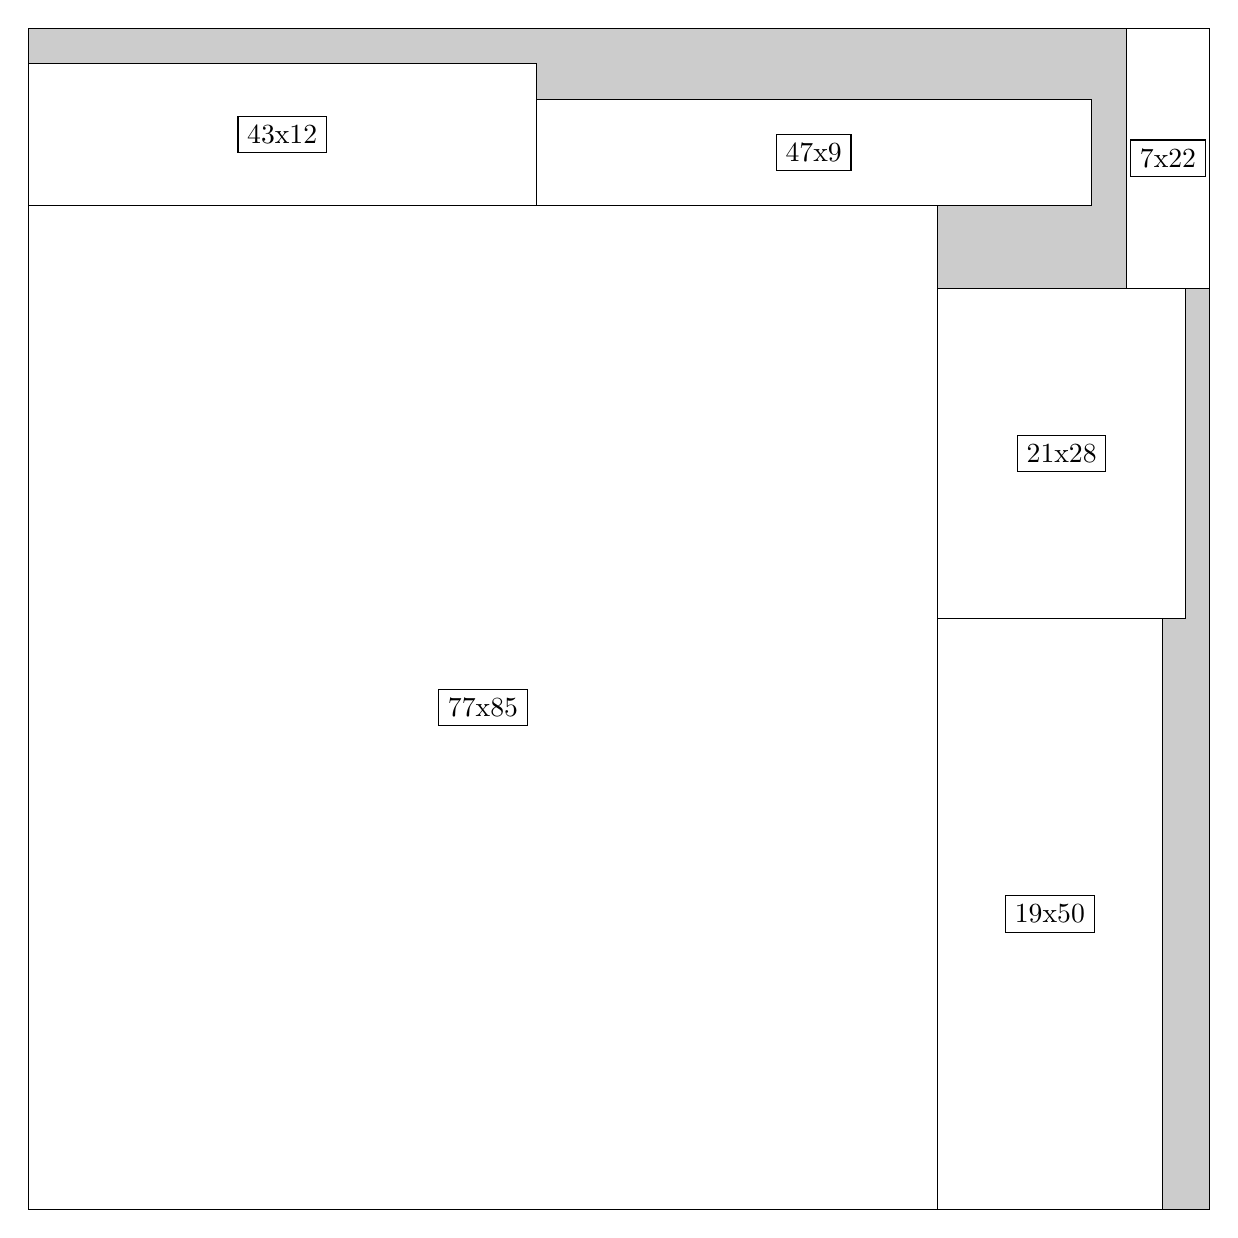
\begin{tikzpicture}[shorten >=1pt,scale=1.0,every node/.style={scale=1.0},->]
\tikzstyle{vertex}=[circle,fill=black!25,minimum size=14pt,inner sep=0pt]
\filldraw[fill=gray!40!white, draw=black] (0,0) rectangle (15.0,15.0);
\foreach \name/\x/\y/\w/\h in {19x50/11.549999999999999/0.0/2.85/7.5,77x85/0.0/0.0/11.549999999999999/12.75,21x28/11.549999999999999/7.5/3.15/4.2,43x12/0.0/12.75/6.45/1.7999999999999998,47x9/6.45/12.75/7.05/1.3499999999999999,7x22/13.95/11.7/1.05/3.3}
\filldraw[fill=white!40!white, draw=black] (\x,\y) rectangle node[draw] (\name) {\name} ++(\w,\h);
\end{tikzpicture}


w =19 , h =50 , x =77 , y =0 , v =950
\par
w =77 , h =85 , x =0 , y =0 , v =6545
\par
w =21 , h =28 , x =77 , y =50 , v =588
\par
w =43 , h =12 , x =0 , y =85 , v =516
\par
w =47 , h =9 , x =43 , y =85 , v =423
\par
w =7 , h =22 , x =93 , y =78 , v =154
\par
\newpage


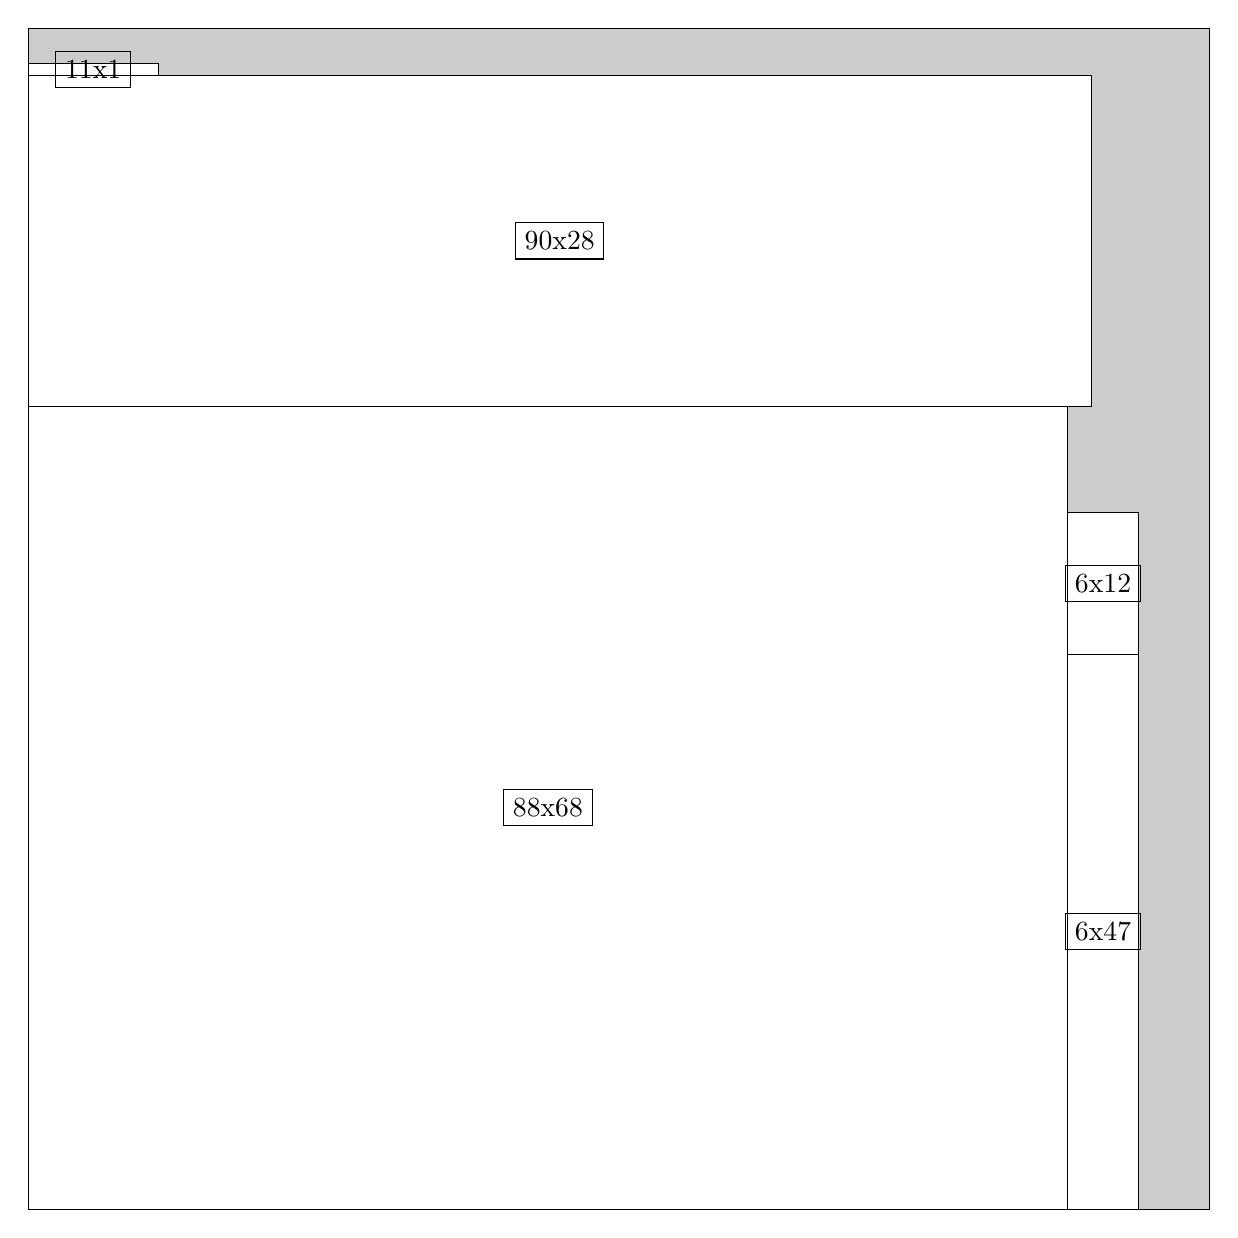
\begin{tikzpicture}[shorten >=1pt,scale=1.0,every node/.style={scale=1.0},->]
\tikzstyle{vertex}=[circle,fill=black!25,minimum size=14pt,inner sep=0pt]
\filldraw[fill=gray!40!white, draw=black] (0,0) rectangle (15.0,15.0);
\foreach \name/\x/\y/\w/\h in {88x68/0.0/0.0/13.2/10.2,90x28/0.0/10.2/13.5/4.2,6x47/13.2/0.0/0.8999999999999999/7.05,6x12/13.2/7.05/0.8999999999999999/1.7999999999999998,11x1/0.0/14.399999999999999/1.65/0.15}
\filldraw[fill=white!40!white, draw=black] (\x,\y) rectangle node[draw] (\name) {\name} ++(\w,\h);
\end{tikzpicture}


w =88 , h =68 , x =0 , y =0 , v =5984
\par
w =90 , h =28 , x =0 , y =68 , v =2520
\par
w =6 , h =47 , x =88 , y =0 , v =282
\par
w =6 , h =12 , x =88 , y =47 , v =72
\par
w =11 , h =1 , x =0 , y =96 , v =11
\par
\newpage


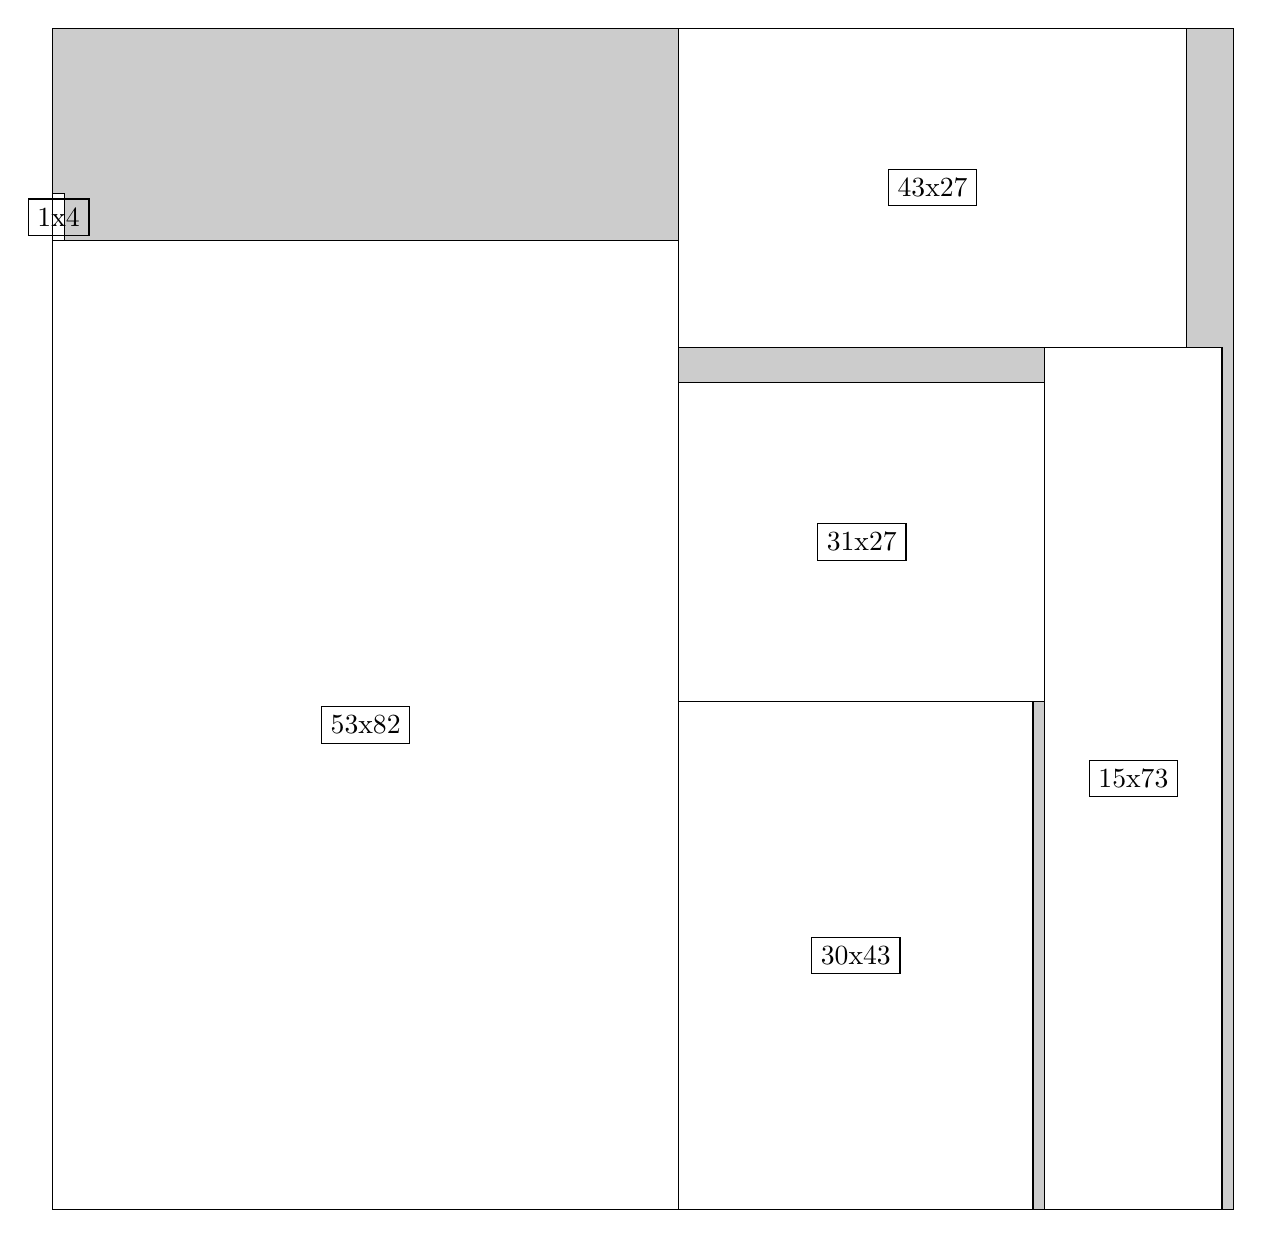
\begin{tikzpicture}[shorten >=1pt,scale=1.0,every node/.style={scale=1.0},->]
\tikzstyle{vertex}=[circle,fill=black!25,minimum size=14pt,inner sep=0pt]
\filldraw[fill=gray!40!white, draw=black] (0,0) rectangle (15.0,15.0);
\foreach \name/\x/\y/\w/\h in {53x82/0.0/0.0/7.949999999999999/12.299999999999999,30x43/7.949999999999999/0.0/4.5/6.45,43x27/7.949999999999999/10.95/6.45/4.05,15x73/12.6/0.0/2.25/10.95,31x27/7.949999999999999/6.45/4.6499999999999995/4.05,1x4/0.0/12.299999999999999/0.15/0.6}
\filldraw[fill=white!40!white, draw=black] (\x,\y) rectangle node[draw] (\name) {\name} ++(\w,\h);
\end{tikzpicture}


w =53 , h =82 , x =0 , y =0 , v =4346
\par
w =30 , h =43 , x =53 , y =0 , v =1290
\par
w =43 , h =27 , x =53 , y =73 , v =1161
\par
w =15 , h =73 , x =84 , y =0 , v =1095
\par
w =31 , h =27 , x =53 , y =43 , v =837
\par
w =1 , h =4 , x =0 , y =82 , v =4
\par
\newpage


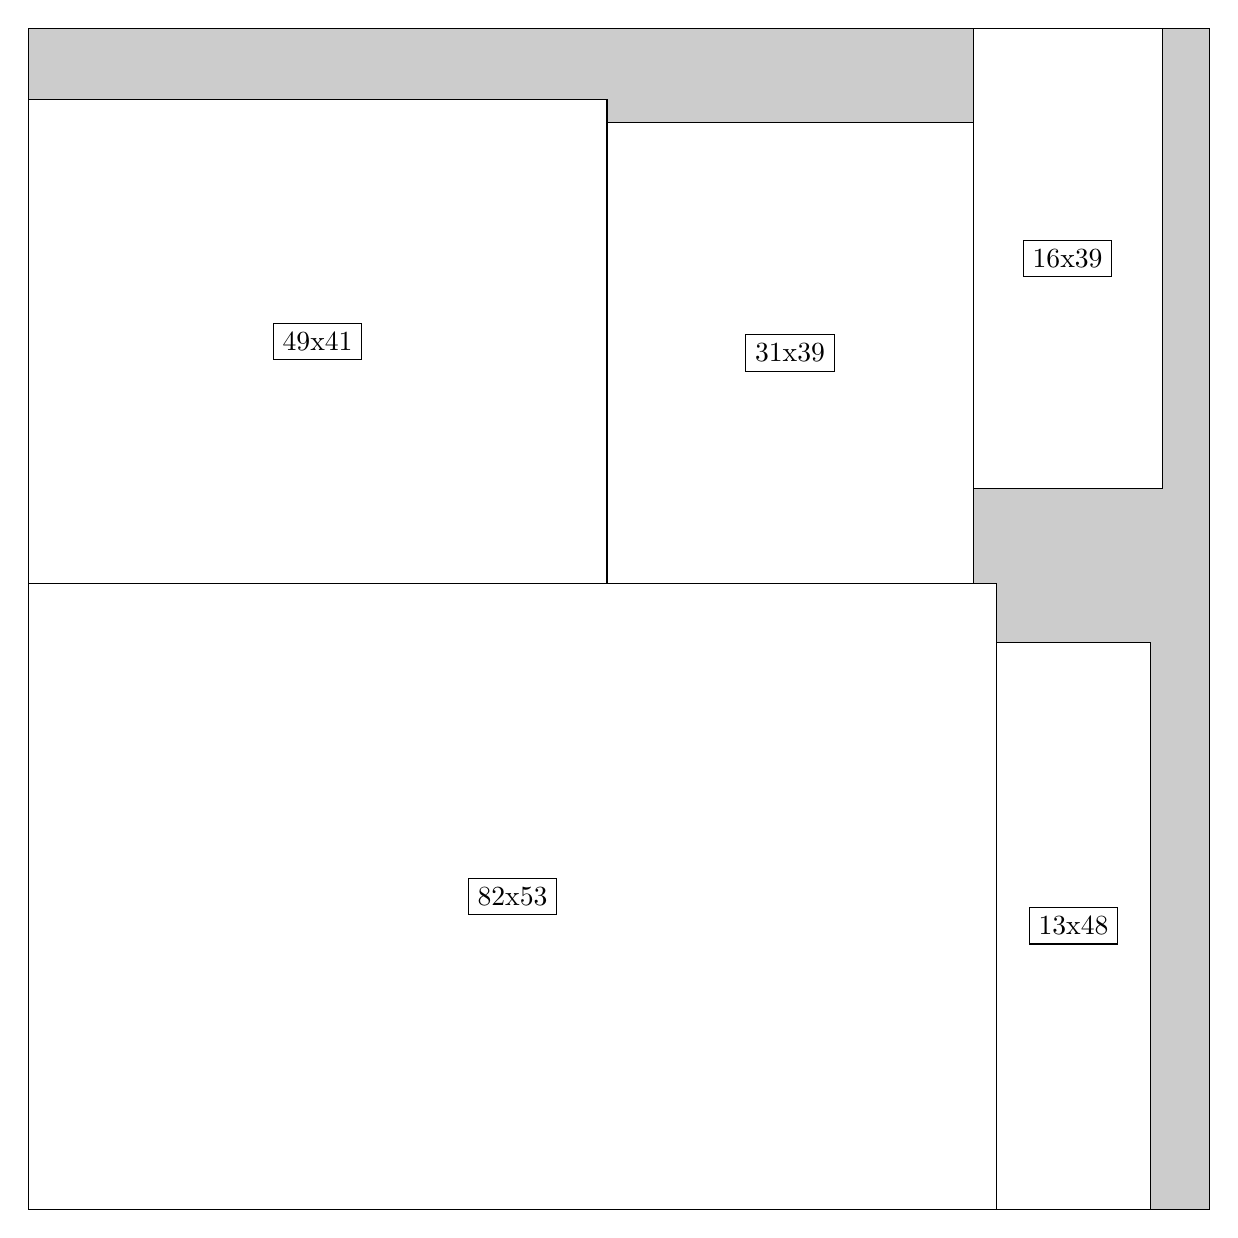
\begin{tikzpicture}[shorten >=1pt,scale=1.0,every node/.style={scale=1.0},->]
\tikzstyle{vertex}=[circle,fill=black!25,minimum size=14pt,inner sep=0pt]
\filldraw[fill=gray!40!white, draw=black] (0,0) rectangle (15.0,15.0);
\foreach \name/\x/\y/\w/\h in {82x53/0.0/0.0/12.299999999999999/7.949999999999999,31x39/7.35/7.949999999999999/4.6499999999999995/5.85,49x41/0.0/7.949999999999999/7.35/6.1499999999999995,13x48/12.299999999999999/0.0/1.95/7.199999999999999,16x39/12.0/9.15/2.4/5.85}
\filldraw[fill=white!40!white, draw=black] (\x,\y) rectangle node[draw] (\name) {\name} ++(\w,\h);
\end{tikzpicture}


w =82 , h =53 , x =0 , y =0 , v =4346
\par
w =31 , h =39 , x =49 , y =53 , v =1209
\par
w =49 , h =41 , x =0 , y =53 , v =2009
\par
w =13 , h =48 , x =82 , y =0 , v =624
\par
w =16 , h =39 , x =80 , y =61 , v =624
\par
\newpage


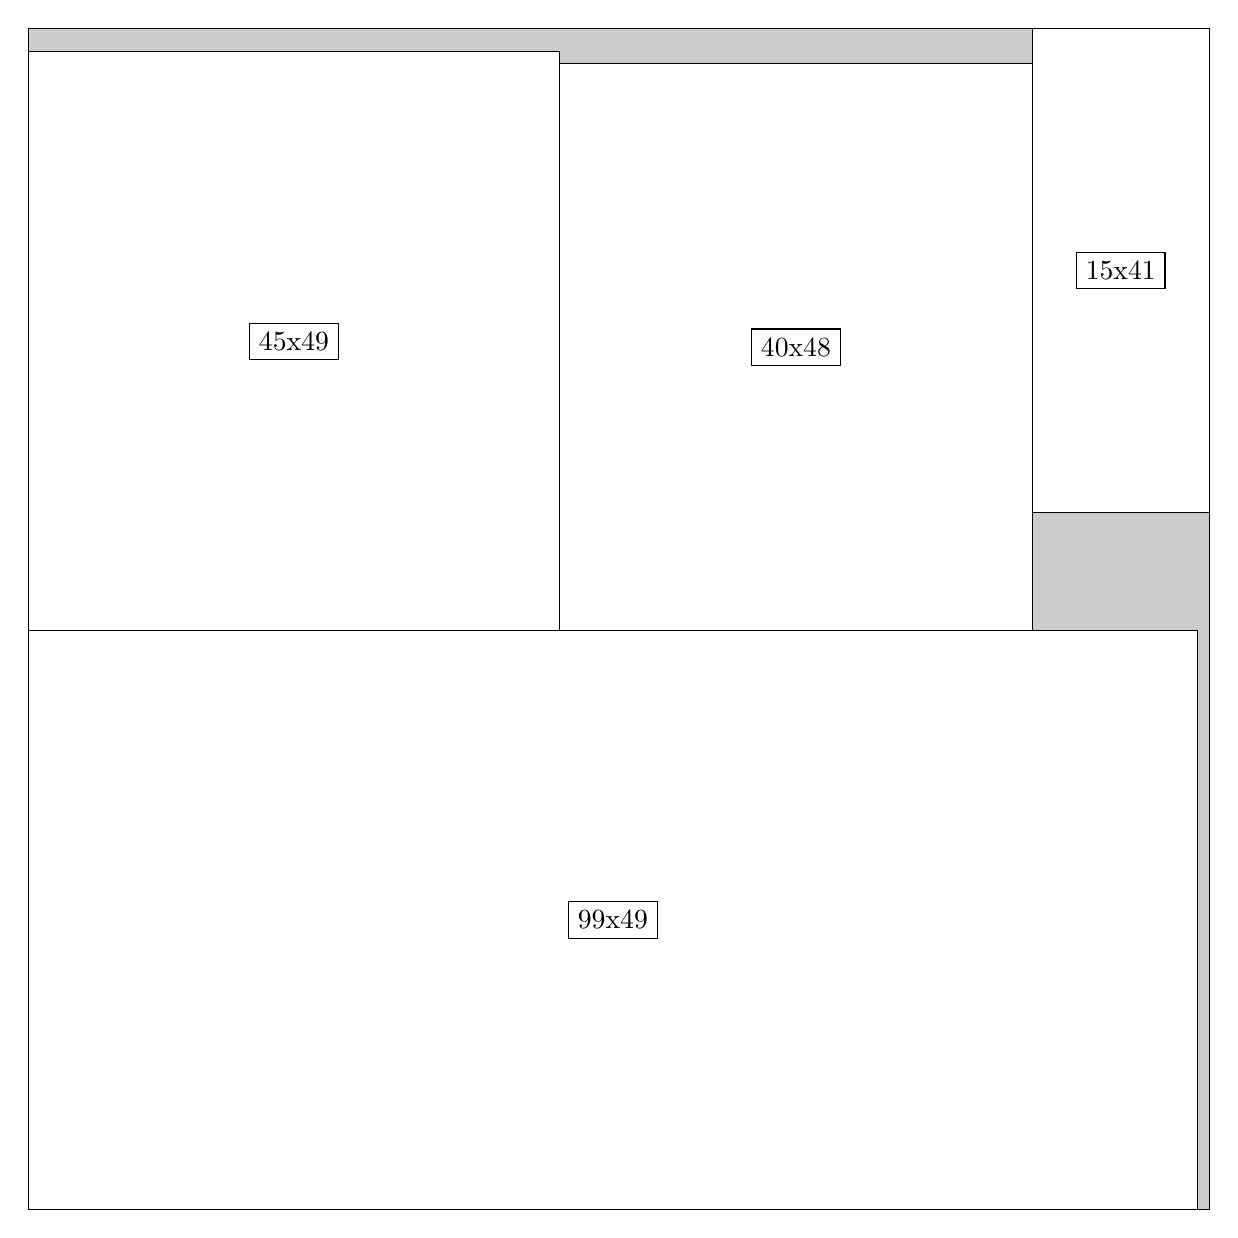
\begin{tikzpicture}[shorten >=1pt,scale=1.0,every node/.style={scale=1.0},->]
\tikzstyle{vertex}=[circle,fill=black!25,minimum size=14pt,inner sep=0pt]
\filldraw[fill=gray!40!white, draw=black] (0,0) rectangle (15.0,15.0);
\foreach \name/\x/\y/\w/\h in {99x49/0.0/0.0/14.85/7.35,45x49/0.0/7.35/6.75/7.35,40x48/6.75/7.35/6.0/7.199999999999999,15x41/12.75/8.85/2.25/6.1499999999999995}
\filldraw[fill=white!40!white, draw=black] (\x,\y) rectangle node[draw] (\name) {\name} ++(\w,\h);
\end{tikzpicture}


w =99 , h =49 , x =0 , y =0 , v =4851
\par
w =45 , h =49 , x =0 , y =49 , v =2205
\par
w =40 , h =48 , x =45 , y =49 , v =1920
\par
w =15 , h =41 , x =85 , y =59 , v =615
\par
\newpage


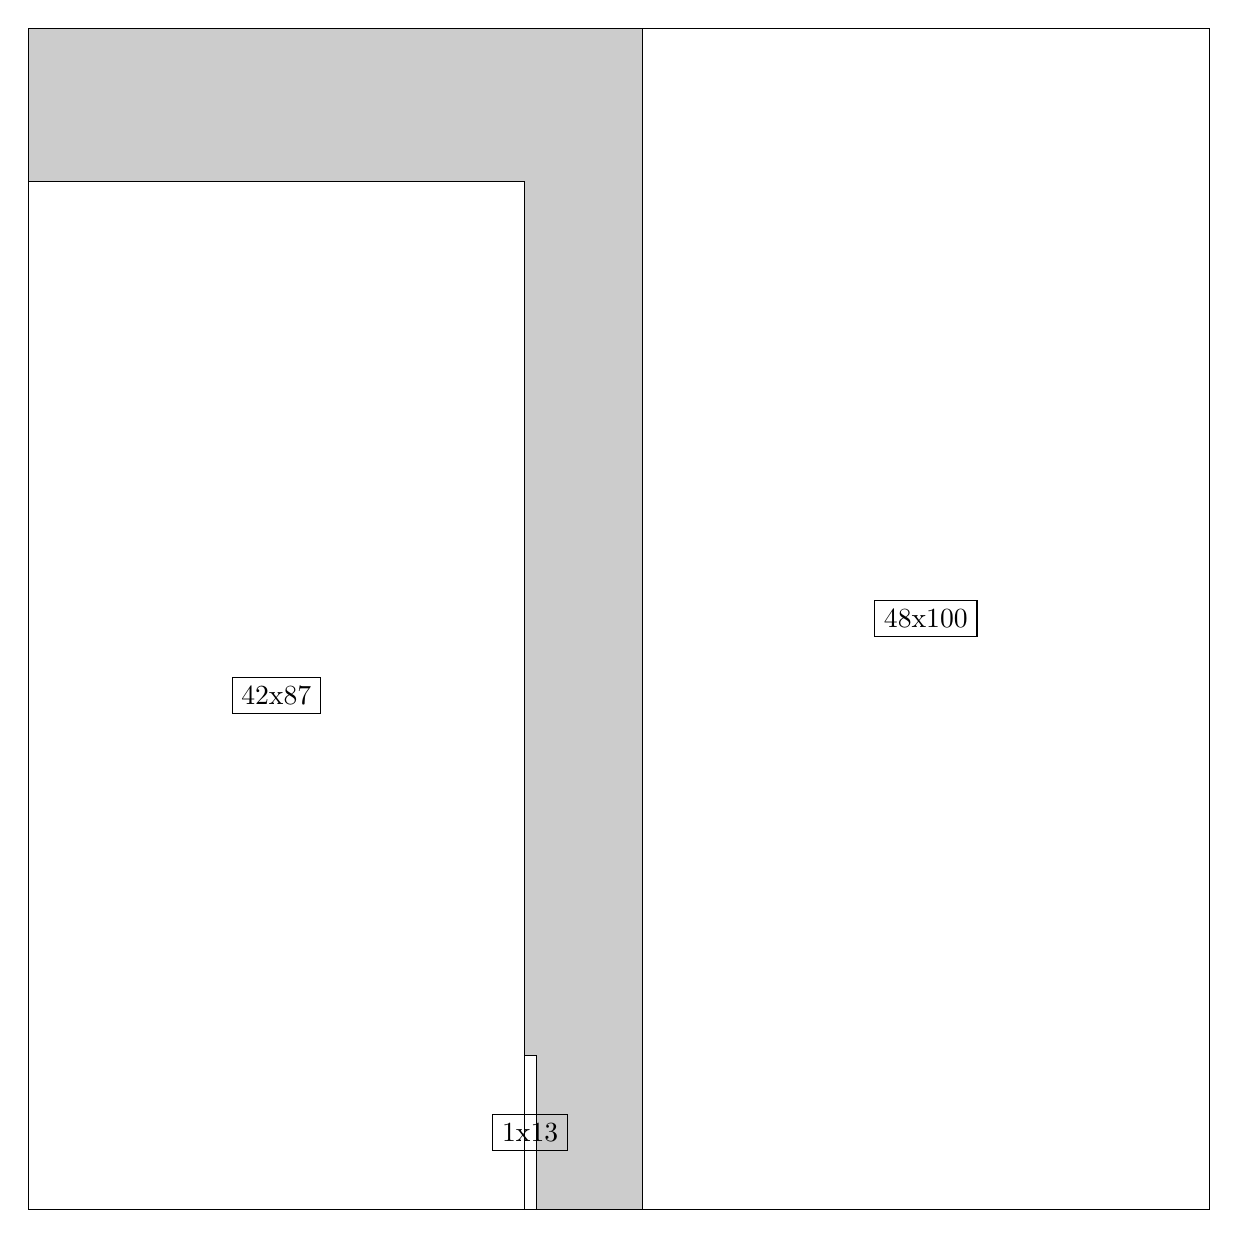
\begin{tikzpicture}[shorten >=1pt,scale=1.0,every node/.style={scale=1.0},->]
\tikzstyle{vertex}=[circle,fill=black!25,minimum size=14pt,inner sep=0pt]
\filldraw[fill=gray!40!white, draw=black] (0,0) rectangle (15.0,15.0);
\foreach \name/\x/\y/\w/\h in {48x100/7.8/0.0/7.199999999999999/15.0,42x87/0.0/0.0/6.3/13.049999999999999,1x13/6.3/0.0/0.15/1.95}
\filldraw[fill=white!40!white, draw=black] (\x,\y) rectangle node[draw] (\name) {\name} ++(\w,\h);
\end{tikzpicture}


w =48 , h =100 , x =52 , y =0 , v =4800
\par
w =42 , h =87 , x =0 , y =0 , v =3654
\par
w =1 , h =13 , x =42 , y =0 , v =13
\par
\newpage


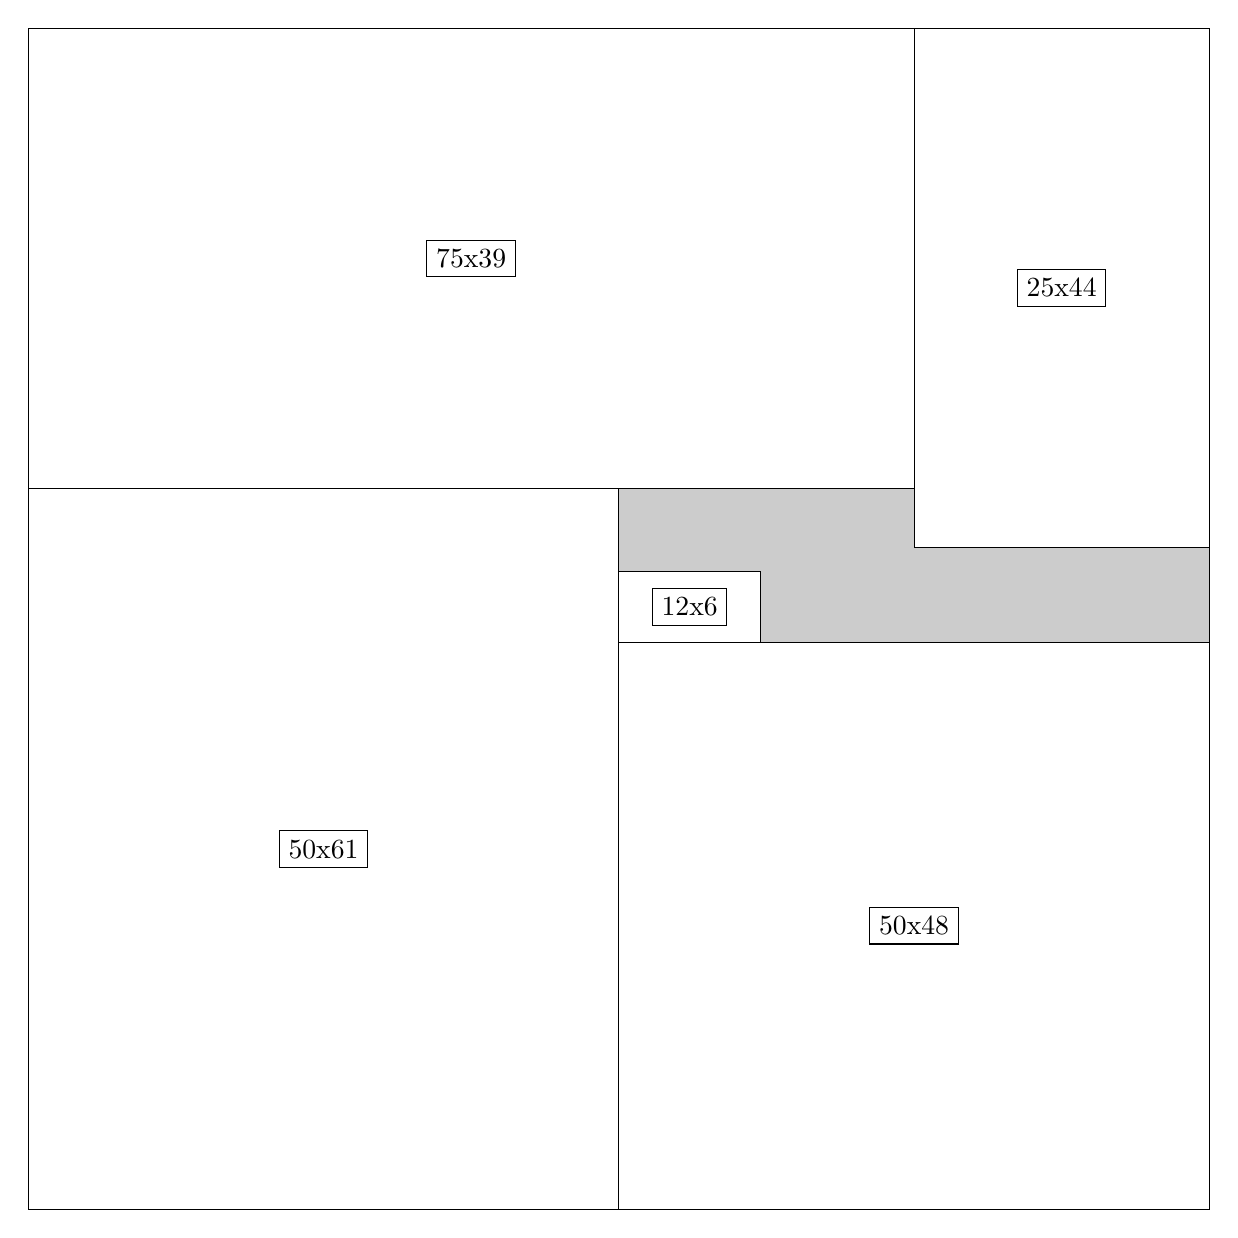
\begin{tikzpicture}[shorten >=1pt,scale=1.0,every node/.style={scale=1.0},->]
\tikzstyle{vertex}=[circle,fill=black!25,minimum size=14pt,inner sep=0pt]
\filldraw[fill=gray!40!white, draw=black] (0,0) rectangle (15.0,15.0);
\foreach \name/\x/\y/\w/\h in {50x61/0.0/0.0/7.5/9.15,75x39/0.0/9.15/11.25/5.85,50x48/7.5/0.0/7.5/7.199999999999999,25x44/11.25/8.4/3.75/6.6,12x6/7.5/7.199999999999999/1.7999999999999998/0.8999999999999999}
\filldraw[fill=white!40!white, draw=black] (\x,\y) rectangle node[draw] (\name) {\name} ++(\w,\h);
\end{tikzpicture}


w =50 , h =61 , x =0 , y =0 , v =3050
\par
w =75 , h =39 , x =0 , y =61 , v =2925
\par
w =50 , h =48 , x =50 , y =0 , v =2400
\par
w =25 , h =44 , x =75 , y =56 , v =1100
\par
w =12 , h =6 , x =50 , y =48 , v =72
\par
\newpage


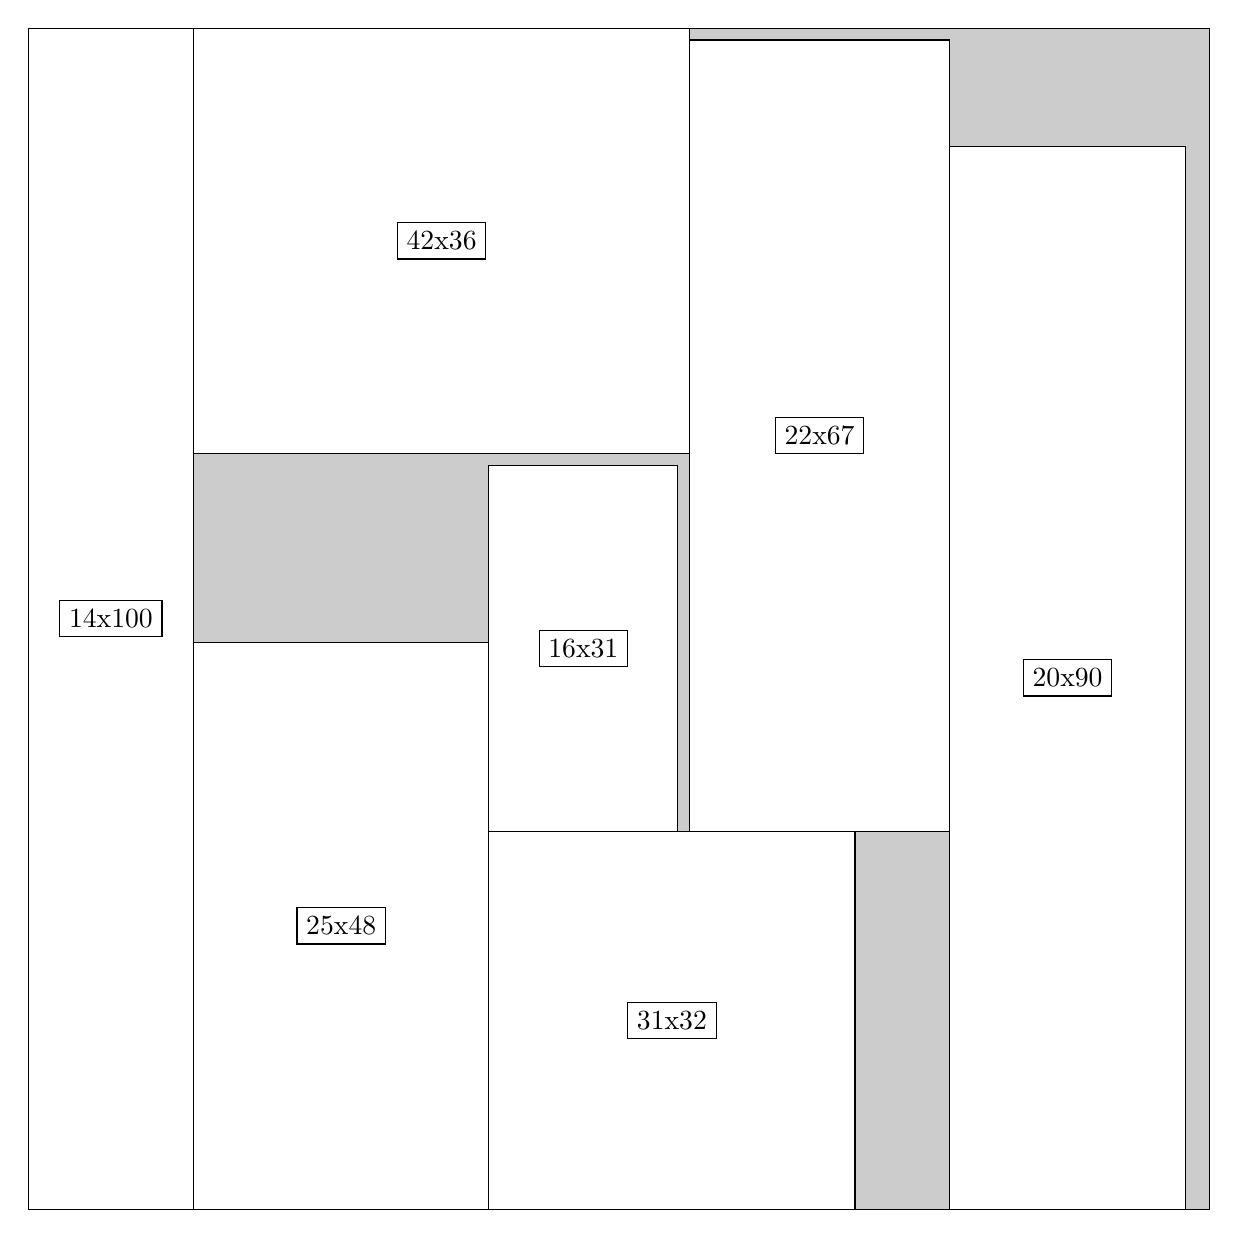
\begin{tikzpicture}[shorten >=1pt,scale=1.0,every node/.style={scale=1.0},->]
\tikzstyle{vertex}=[circle,fill=black!25,minimum size=14pt,inner sep=0pt]
\filldraw[fill=gray!40!white, draw=black] (0,0) rectangle (15.0,15.0);
\foreach \name/\x/\y/\w/\h in {25x48/2.1/0.0/3.75/7.199999999999999,20x90/11.7/0.0/3.0/13.5,42x36/2.1/9.6/6.3/5.3999999999999995,22x67/8.4/4.8/3.3/10.049999999999999,14x100/0.0/0.0/2.1/15.0,31x32/5.85/0.0/4.6499999999999995/4.8,16x31/5.85/4.8/2.4/4.6499999999999995}
\filldraw[fill=white!40!white, draw=black] (\x,\y) rectangle node[draw] (\name) {\name} ++(\w,\h);
\end{tikzpicture}


w =25 , h =48 , x =14 , y =0 , v =1200
\par
w =20 , h =90 , x =78 , y =0 , v =1800
\par
w =42 , h =36 , x =14 , y =64 , v =1512
\par
w =22 , h =67 , x =56 , y =32 , v =1474
\par
w =14 , h =100 , x =0 , y =0 , v =1400
\par
w =31 , h =32 , x =39 , y =0 , v =992
\par
w =16 , h =31 , x =39 , y =32 , v =496
\par
\newpage


\end{document}